\section{Benchmark}

\subsection{lmapper VS kmapper}
We benchmarked lmapper against Kepler Mapper. To benchmark it a specific cover was implemented in \lstinline|lmapper.cover.KeplerCover| in order to implement the same method to build the cover. In both cases the filter used is a projection, since Kepler Mapper do not implement the Eccentricity filter. For this reason it is not possible to take advantage of the \lstinline|filterutils| package. As a clustering algorithm it was used a single linkage algorithm, where for lmapper the \lstinline|cutoff.FirstGap| class has been used to find the number of clusters, whereas for kmapper it was only possible to set a predetermined number of clusters, that has been chosen to be 2. Note that the performances of \lstinline|lmapper| are highly dependent on the parameter chosen to initialize \lstinline|cutoff.FirstGap|. Specifically, the smaller the parameter, the more clusters will be created and the slower will be the method \lstinline|complex.Complex.fit| affecting the overall performances of the package. For this benchmark this parameter has been set in order to obtain a graph the most similar to the one obtained by Kepler Mapper.

\textbf{Hardware used}:
Mac Book Pro late 2011 13", with a 32 nm "Sandy Bridge" 2.4 GHz Intel "Core i5" processor (2435M), 8 GB of 1333 MHz DDR3 SDRAM in two modules of 4GB each.

\begin{figure}[h]
	\caption{Performance comparison}
	\centering
	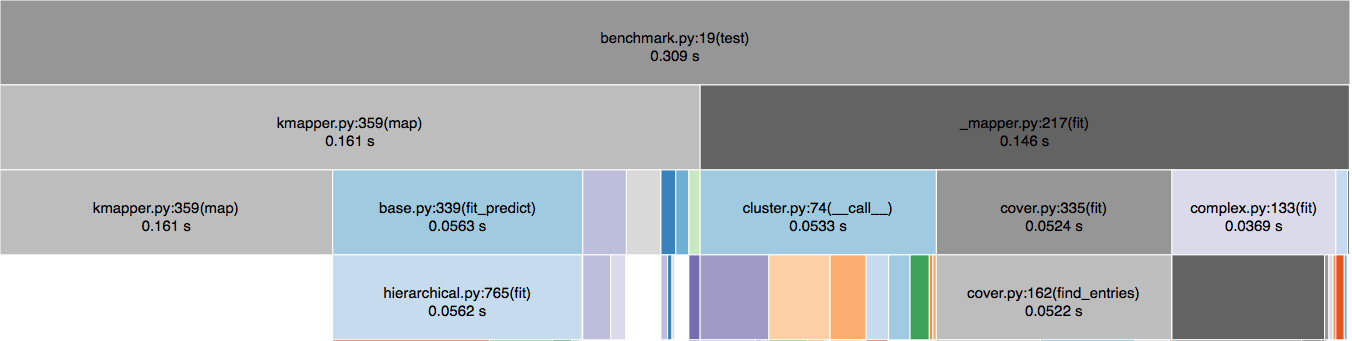
\includegraphics[width=0.9\textwidth]{images/benchmark/synthetic/benchmark}
\end{figure}
\begin{figure}[h]
	\caption{Graph obtained with Kepler Mapper}
	\centering
	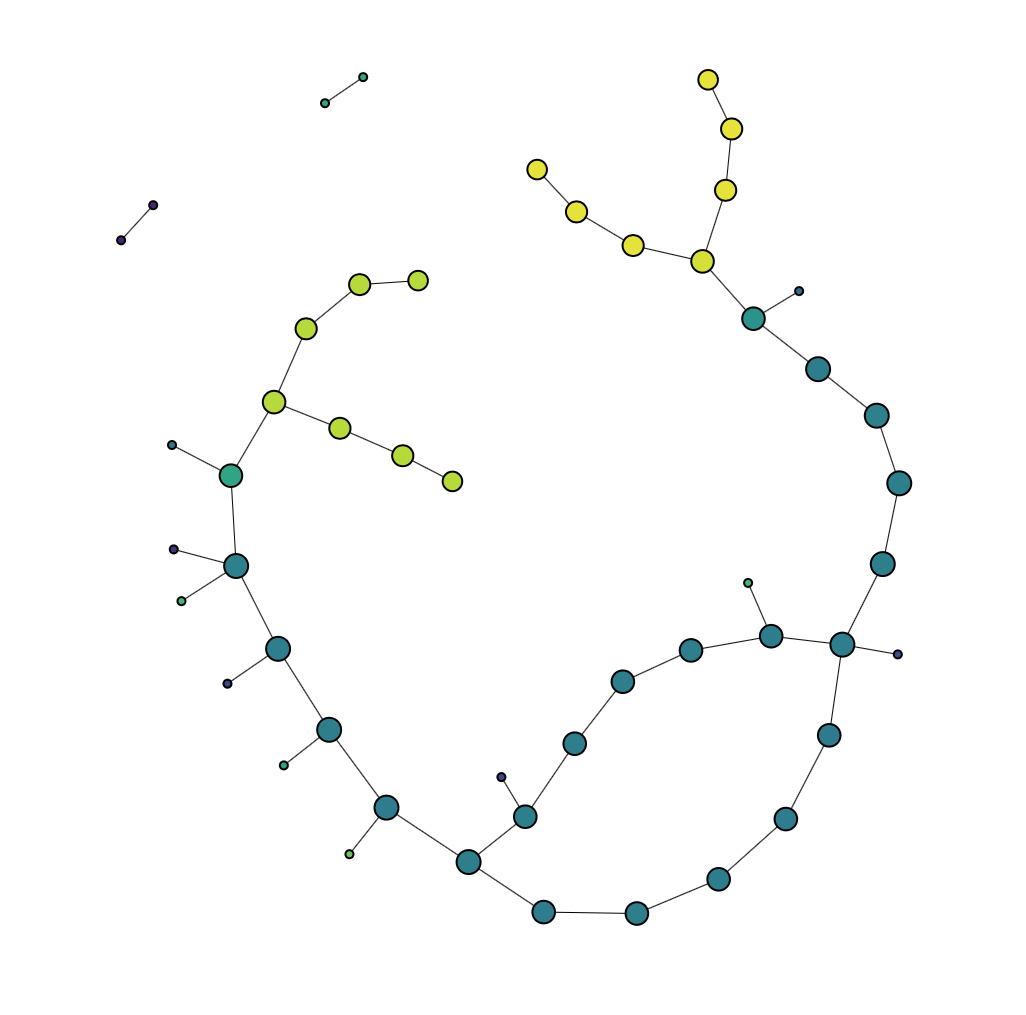
\includegraphics[width=0.5\textwidth]{images/benchmark/synthetic/benchmark_kmapper}
\end{figure}
\begin{figure}[h]
	\caption{Result obtained with lmapper}
	\centering
	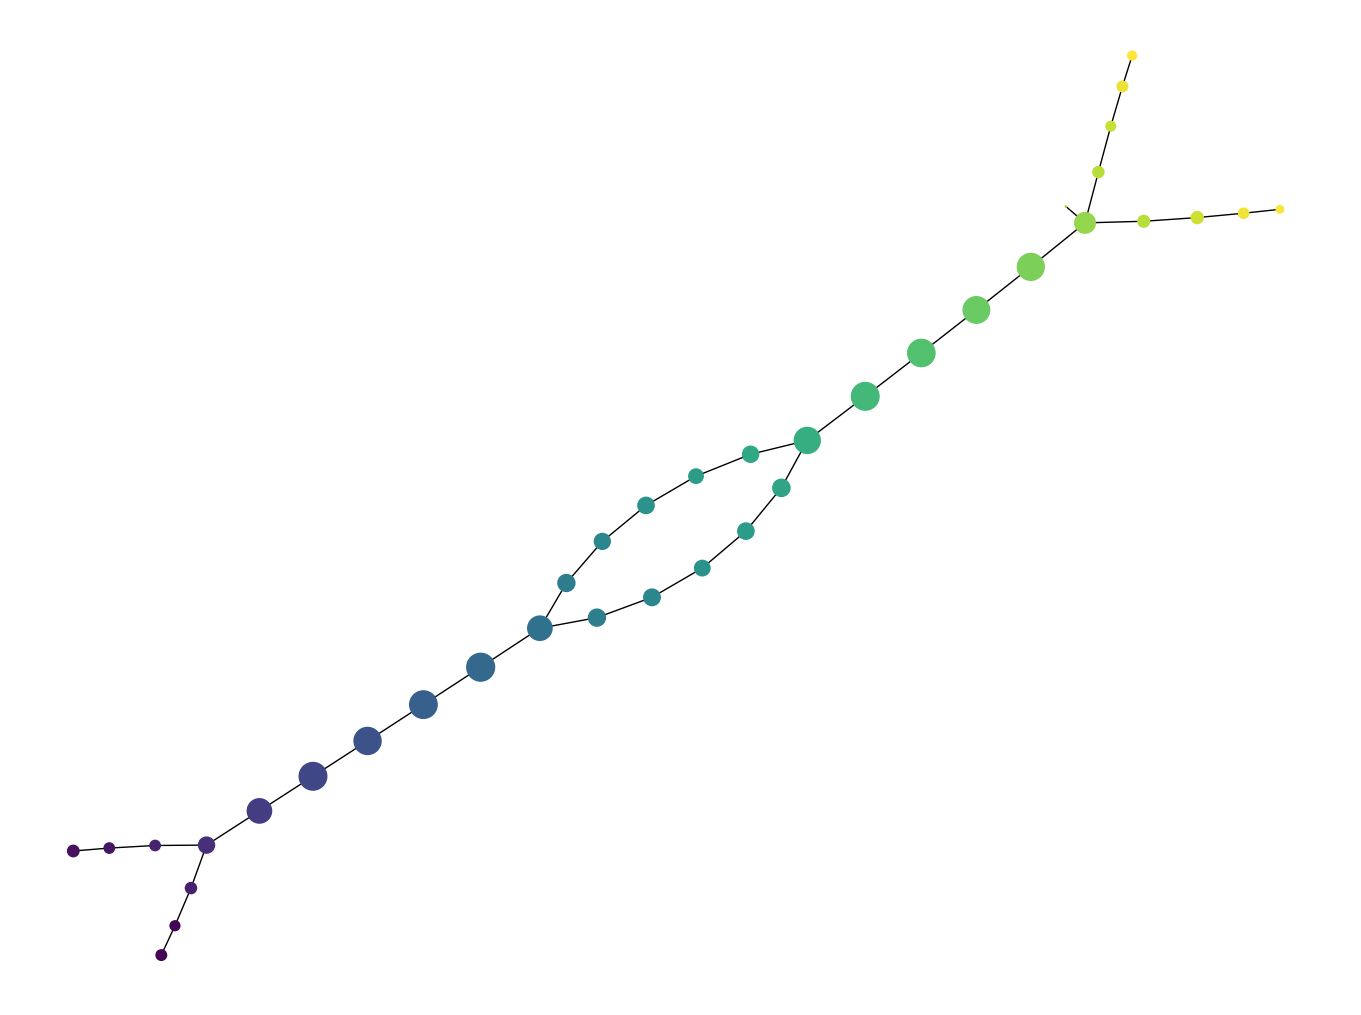
\includegraphics[width=0.5\textwidth]{images/benchmark/synthetic/benchmark_lmapper}
\end{figure}

\begin{figure}[h]
	\caption{Performance comparison}
	\centering
	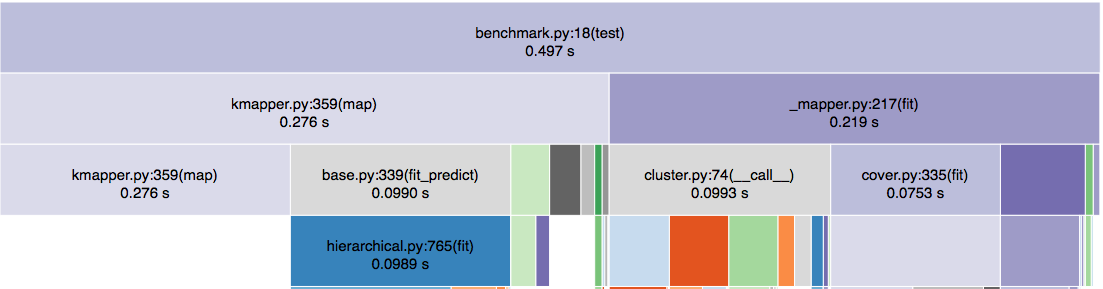
\includegraphics[width=0.9\textwidth]{images/benchmark/cat/benchmark}
\end{figure}
\begin{figure}[h]
	\caption{Graph obtained with Kepler Mapper}
	\centering
	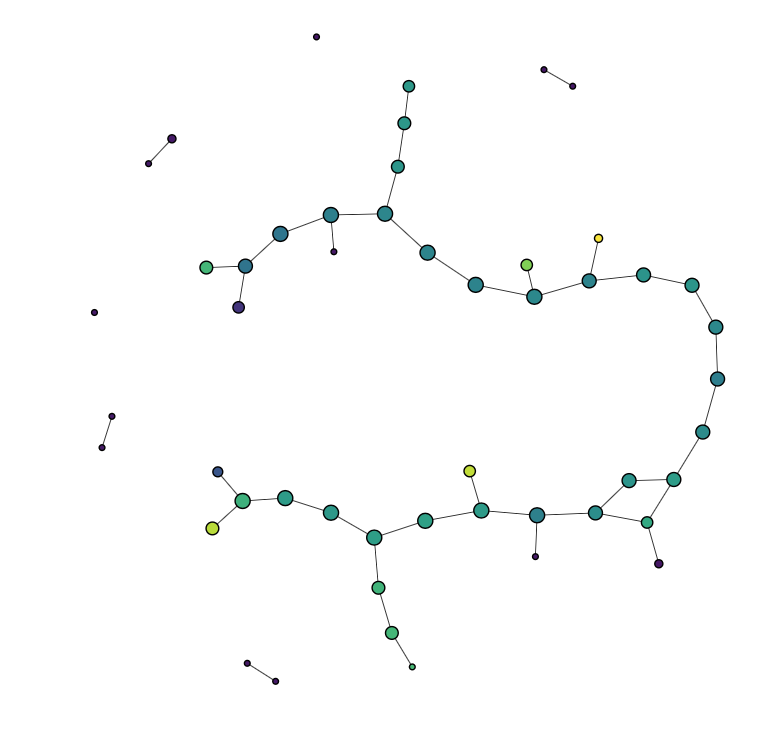
\includegraphics[width=0.5\textwidth]{images/benchmark/cat/benchmark_kmapper}
\end{figure}
\begin{figure}[h]
	\caption{Result obtained with lmapper}
	\centering
	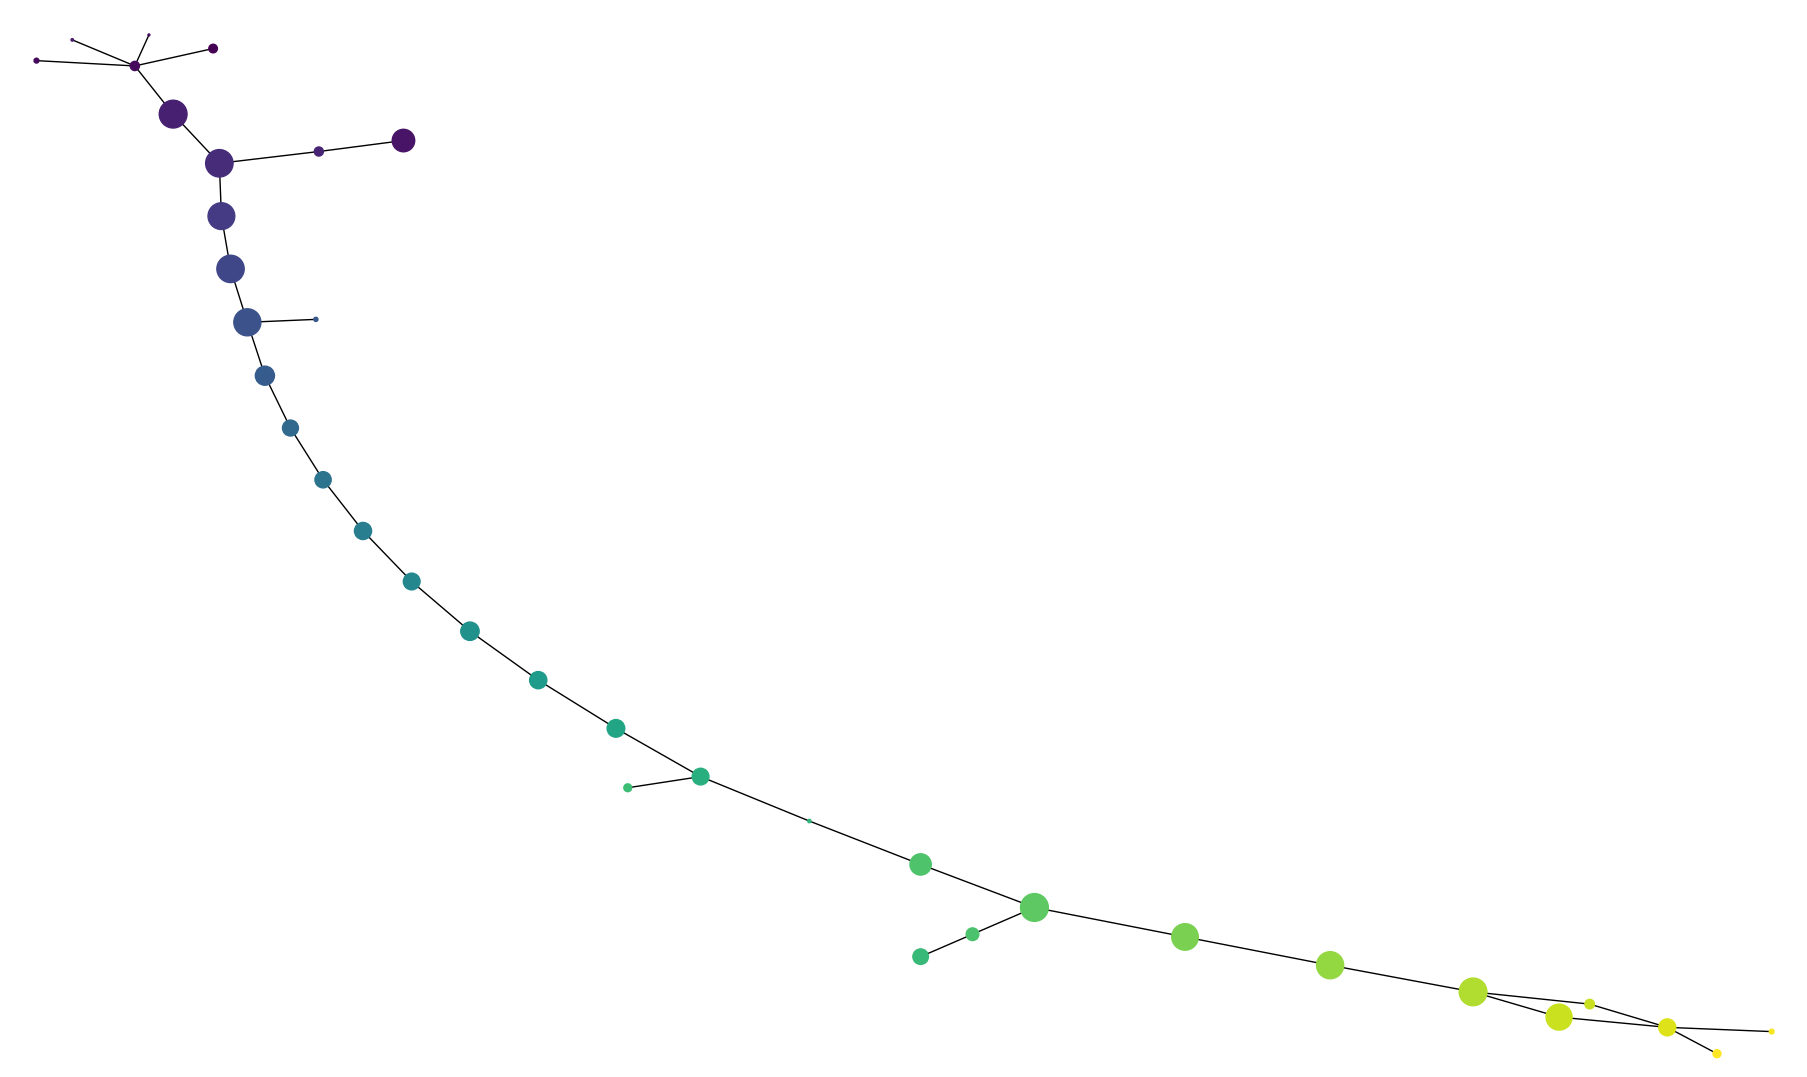
\includegraphics[width=0.5\textwidth]{images/benchmark/cat/benchmark_lmapper}
\end{figure}

\paragraph{Conclusions}
The pure Python implementation obtained a speedup of 10\% and 20\% compared to Kepler Mapper on the synthetic dataset of Palma and the Cat dataset of \cite{pythonmapper}.


\subsection{filterutils}
\paragraph{Conclusions}
We see that the package filterutils.cpp managed to get an almost perfect speedup, almost linear with the number of threads launched.

\subsection{predmap}

\paragraph{Conclusions}
We managed to obtain the same results of Francesco Palma's masther thesis